\documentclass[11pt,a4paper]{article}

% 中文支持
\usepackage[scheme=plain]{ctex}
% 页面设置
\usepackage[margin=2.5cm]{geometry}
% 数学公式与符号（mathtools 会加载 amsmath 并提供 \coloneqq）
\usepackage{mathtools}
\usepackage{amssymb}
% 图表
\usepackage{graphicx}
\usepackage{subcaption}
\usepackage{booktabs}
\usepackage{multirow}
\usepackage{array}
% 超链接
\usepackage{hyperref}
% 算法伪代码
\usepackage{algorithm}
\usepackage{algpseudocode}

% 自定义命令
\newcommand{\dsai}{DeepSeek-AI}
\newcommand{\dsvfour}{DeepSeek-V4}
\newcommand{\dsvfourpro}{DeepSeek-V4-Pro}
\newcommand{\dsvfourflash}{DeepSeek-V4-Flash}
\newcommand{\dsvfourpromax}{DeepSeek-V4-Pro-Max}
\newcommand{\dsvfourflashmax}{DeepSeek-V4-Flash-Max}
\newcommand{\dsvthree}{DeepSeek-V3}
\newcommand{\dsvthreetwo}{DeepSeek-V3.2}
\newcommand{\moe}{MoE}

\title{\dsvfour：迈向高效百万级Token上下文智能}
\author{深度求索人工智能研究室 \\ \texttt{research@deepseek.com}}
\date{\today}

\begin{document}

\maketitle

\begin{abstract}
我们在此呈现\dsvfour 系列的预览版本，该系列包含两个强大的混合专家（Mixture-of-Experts, \moe{}）语言模型——拥有1.6万亿参数（49B激活）的\dsvfourpro 以及拥有2840亿参数（13B激活）的\dsvfourflash——两者均支持一百万Token的上下文长度。\dsvfour 系列在架构和优化方面融合了若干关键升级：（1）结合了压缩稀疏注意力（CSA）与重度压缩注意力（HCA）的混合注意力架构，以提升长上下文效率；（2）用于增强传统残差连接的流形约束超连接（mHC）；（3）以及用于更快收敛和更强训练稳定性的Muon优化器。我们在超过32万亿个多样化且高质量的Token上对两个模型进行了预训练，随后进行了全面的后训练流程，以释放并进一步增强其能力。作为\dsvfourpro 的最大推理努力模式，\dsvfourpromax 重新定义了开源模型的技术前沿，在核心任务上超越了其前代模型。同时，\dsvfour 系列在长上下文场景中极其高效。在一百万Token上下文的设定下，与\dsvthreetwo 相比，\dsvfourpro 的单Token推理FLOPs仅为其\(27\%\)，KV缓存仅为其\(10\%\)。这使我们能够常规地支持一百万Token的上下文，从而使长程任务和进一步的测试时扩展变得更为可行。模型检查点可在 \url{https://huggingface.co/collections/deepseek-ai/deepseek-v4} 获取。
\end{abstract}

\begin{figure}[H]
\centering
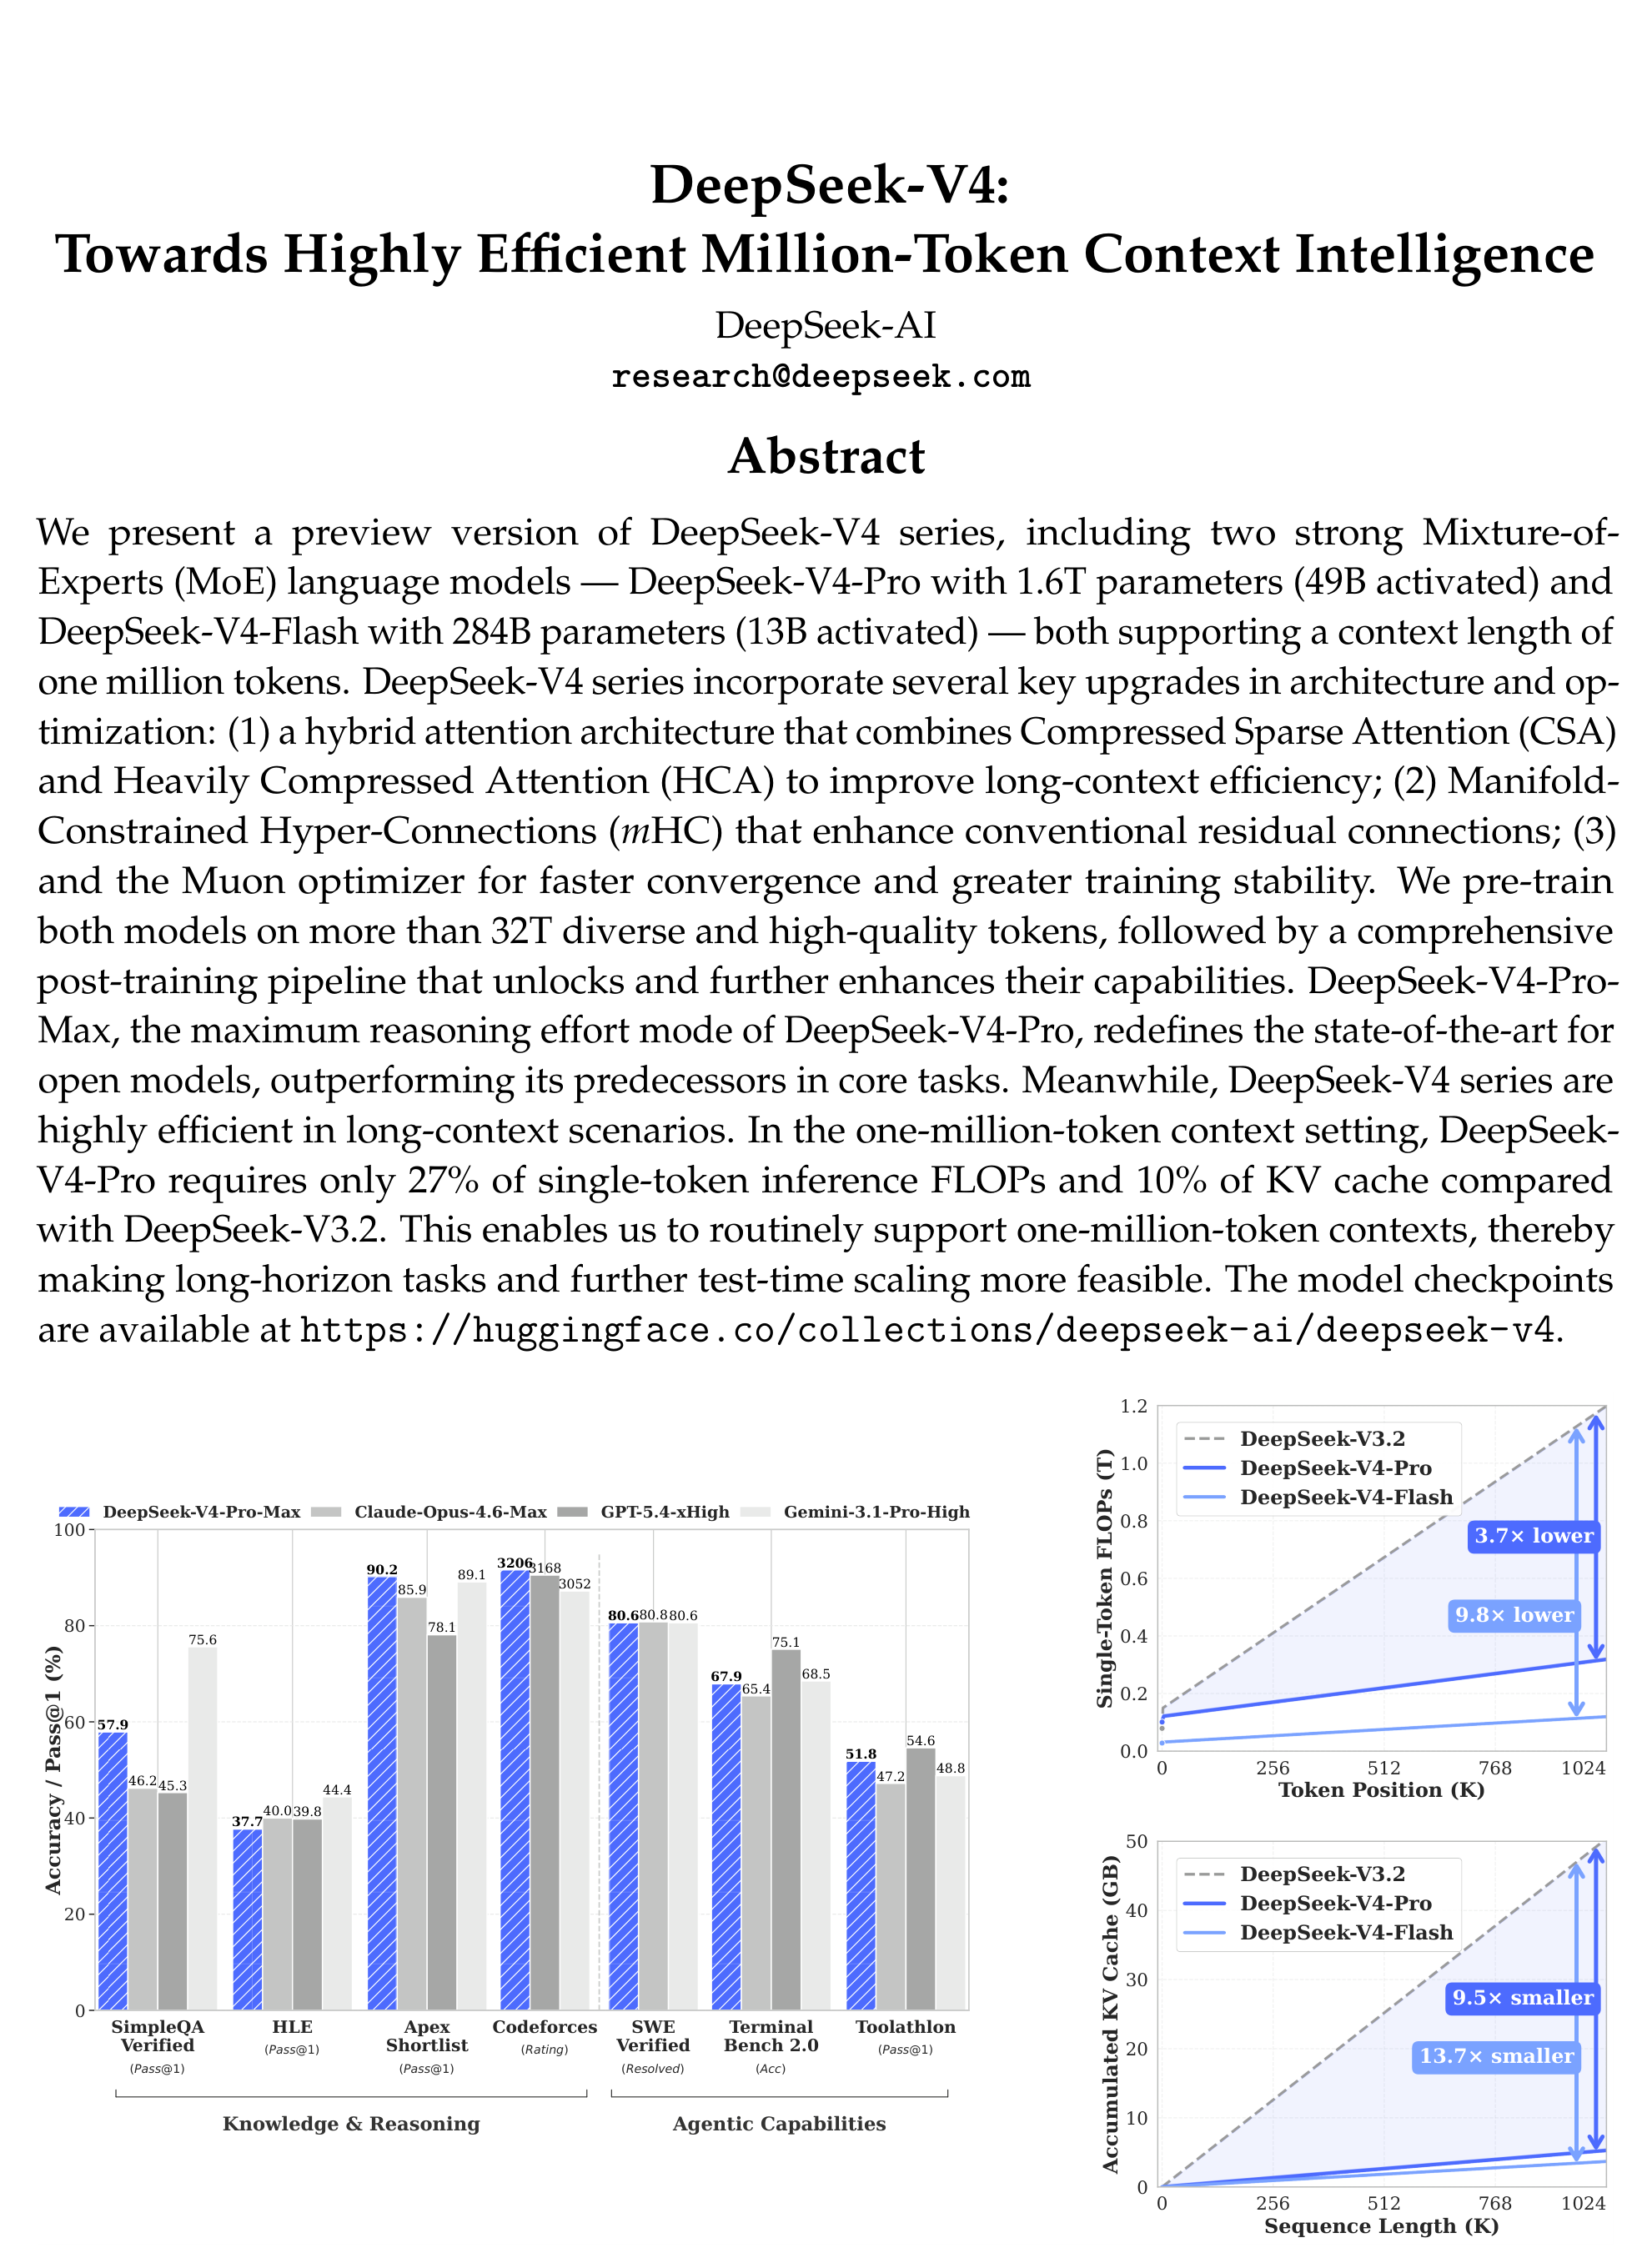
\includegraphics[width=\textwidth]{figures/DeepSeek_V4_fig01.png}
\caption{\dsvfourpromax 与同类模型的基准性能对比。左图：标准基准性能比较。右图：推理效率对比。}
\label{fig:overview}
\end{figure}

% ===== 1. 引言 =====
\section{引言}

推理模型的出现，确立了测试时扩展的新范式，为大语言模型带来了显著的性能提升。然而，这种扩展范式从根本上受到传统注意力机制二次计算复杂度的制约，这为超长上下文和推理过程制造了一个难以逾越的瓶颈。与此同时，从复杂的智能体工作流到海量跨文档分析等长程场景和任务的出现，也使得对超长上下文的高效支持对未来发展至关重要。尽管近期的一些开源工作在提升通用能力方面取得了进展，但在处理超长序列时，核心架构效率低下的问题仍然是关键障碍，限制了测试时扩展的进一步收益，并阻碍了对长程场景和任务的深入探索。

为了打破超长上下文中的效率壁垒，我们开发了\dsvfour 系列。通过架构创新，\dsvfour 系列在处理超长序列的计算效率上实现了巨大飞跃。这一突破使得对一百万Token上下文长度的高效支持成为可能，为下一代大语言模型开创了百万级上下文的新纪元。我们相信，我们高效处理超长序列的能力解锁了测试时扩展的下一个前沿，为深入研究长程任务铺平了道路，并为探索诸如在线学习等未来范式建立了必要基础。

与\dsvthree 架构相比，\dsvfour 系列保留了DeepSeekMoE框架和多Token预测策略，同时在架构和优化方面引入了多项关键创新。为了增强长上下文效率，我们设计了一种结合了压缩稀疏注意力（CSA）和重度压缩注意力（HCA）的混合注意力机制。CSA沿序列维度压缩KV缓存，然后执行DeepSeek稀疏注意力，而HCA则对KV缓存进行更激进的压缩，但保持密集注意力。为了加强建模能力，我们融合了流形约束超连接，对传统残差连接进行升级。此外，我们将Muon优化器引入到\dsvfour 系列的训练中，从而实现了更快的收敛和更强的训练稳定性。

为了实现\dsvfour 系列的高效训练和推理以及富有成效的开发，我们引入了若干基础设施优化。首先，我们为\moe{}模块设计并实现了一个单一的融合内核，全面重叠了计算、通信和内存访问。其次，我们采用了领域特定语言TileLang来平衡开发效率和运行时效率。第三，我们提供了高效的批次不变和确定性内核库，确保跨训练和推理的逐位可复现性。第四，我们对\moe{}专家权重和索引器QK路径采用FP4量化感知训练，以减少内存和计算量。第五，在训练框架方面，我们扩展了自动微分框架，加入了张量级检查点以实现精细的重计算控制；并通过针对Muon优化器的混合ZeRO策略、通过重计算和融合内核对mHC进行高性价比实现，以及用于管理压缩注意力的两阶段上下文并行，提升了训练效率。最后，在推理框架方面，我们设计了一种异构KV缓存结构，并配有磁盘存储策略，以实现高效的共享前缀复用。

通过采用混合CSA和HCA，以及计算和存储上的精度优化，与\dsvthreetwo 相比，\dsvfour 系列实现了显著更低的推理FLOPs和大幅减少的KV缓存大小，尤其是在长上下文设置下。在一百万Token上下文的场景下，即使是拥有更大激活参数量的\dsvfourpro，其单Token FLOPs也仅为\dsvthreetwo 的\(27\%\)，KV缓存大小仅为其\(10\%\)。此外，\dsvfourflash 凭借其较小的激活参数量，进一步提升了效率：在1M上下文设定下，其单Token FLOPs仅为\dsvthreetwo 的\(10\%\)，KV缓存大小仅为其\(7\%\)。此外，对于\dsvfour 系列，通往专家参数的路径采用FP4精度。虽然目前FP4 × FP8运算的峰值FLOPs与FP8 × FP8相同，但在未来硬件上理论上可以实现1/3的效率提升，这将进一步增强\dsvfour 系列的效率。

\dsvfour-Pro-Base将进一步扩展这一优势，在DeepSeek基础模型中树立新的性能标准，在推理、编码、长上下文和世界知识等任务上达到可比的性能。

\subsection*{核心评估结果摘要}
\begin{itemize}
    \item \textbf{知识}：在广泛的世界知识评估中，\dsvfourpromax 在SimpleQA和Chinese-SimpleQA基准上显著优于领先的开源模型。关于教育知识——通过MMLU-Pro、HLE和GPQA评估——\dsvfourpromax 相较于其开源同行显示出微弱领先。\dsvfourpromax 已显著缩小了与领先闭源模型Gemini-3.1-Pro的差距，尽管在这些基于知识的评估中仍落后于它。
    \item \textbf{推理}：通过推理Token的扩展，\dsvfourpromax 在标准推理基准上展现出优于GPT-5.2和Gemini-3.0-Pro的性能。尽管如此，其性能仍略逊于GPT-5.4和Gemini-3.1-Pro，这表明其发展轨迹落后于前沿顶级模型约3至6个月。此外，\dsvfourflashmax 取得了与GPT-5.2和Gemini-3.0-Pro相当的性能，确立了其作为复杂推理任务中高性价比架构的地位。
    \item \textbf{智能体}：在公开基准上，\dsvfourpromax 与Kimi-K2.6和GLM-5.1等领先开源模型持平，但略逊于前沿闭源模型。在我们的内部评估中，\dsvfourpromax 超越了Claude Sonnet 4.5，并接近Opus 4.5的水平。
    \item \textbf{长上下文}：\dsvfourpromax在1M上下文窗口的合成和真实用例中表现出色，在学术基准上甚至超越了Gemini-3.1-Pro。
    \item \textbf{Pro vs. Flash}：由于参数规模较小，\dsvfourflashmax 在知识评估中表现较低。然而，当分配更大的思考预算时，它在推理任务上取得了可比的结果。在智能体评估中，虽然\dsvfourflashmax 在若干基准上匹配了\dsvfourpromax 的性能，但在更复杂、高难度的任务上仍落后于其更大的兄弟模型。
\end{itemize}

% ===== 2. 架构 =====
\section{架构}

总体而言，\dsvfour 系列保留了Transformer架构和多Token预测模块，同时相较于\dsvthree 引入了几项关键升级：（1）首先，我们引入流形约束超连接（mHC）以增强传统的残差连接；（2）其次，我们设计了一种混合注意力架构，通过压缩稀疏注意力和重度压缩注意力极大地提高了长上下文效率；（3）第三，我们采用Muon作为优化器。对于混合专家组件，我们仍采用DeepSeekMoE架构，仅对\dsvthree 进行了微小调整。多Token预测配置与\dsvthree 保持一致。所有其他未指明的细节均遵循\dsvthree 建立的设置。

\subsection{承继自DeepSeek-V3的设计}

\textbf{混合专家}。与之前的DeepSeek系列模型一样，\dsvfour 系列也为前馈网络采用了DeepSeekMoE范式，该范式设置了细粒度的路由专家和共享专家。与\dsvthree 不同的是，我们将计算亲和力分数的激活函数从Sigmoid改为\(\sqrt{\text{Softplus}(\cdot)}\)。对于负载均衡，我们也采用无辅助损失策略，并辅以轻微的序列级平衡损失，以防止单个序列内的极端失衡。对于\dsvfour，我们移除了对路由目标节点数量的限制，并仔细重新设计了并行策略以保持训练效率。此外，与\dsvthree 相比，我们将最初几个Transformer块中的密集FFN层替换为采用哈希路由的\moe{}层。哈希路由策略根据输入Token ID，依照预定义的哈希函数确定每个Token的目标专家。

\textbf{多Token预测}。如同\dsvthree，\dsvfour 系列也设置了多Token预测模块和目标。鉴于该策略已在\dsvthree 中得到验证，我们对\dsvfour 系列采用相同策略且未作修改。

\subsection{流形约束超连接}

\begin{figure}[H]
\centering
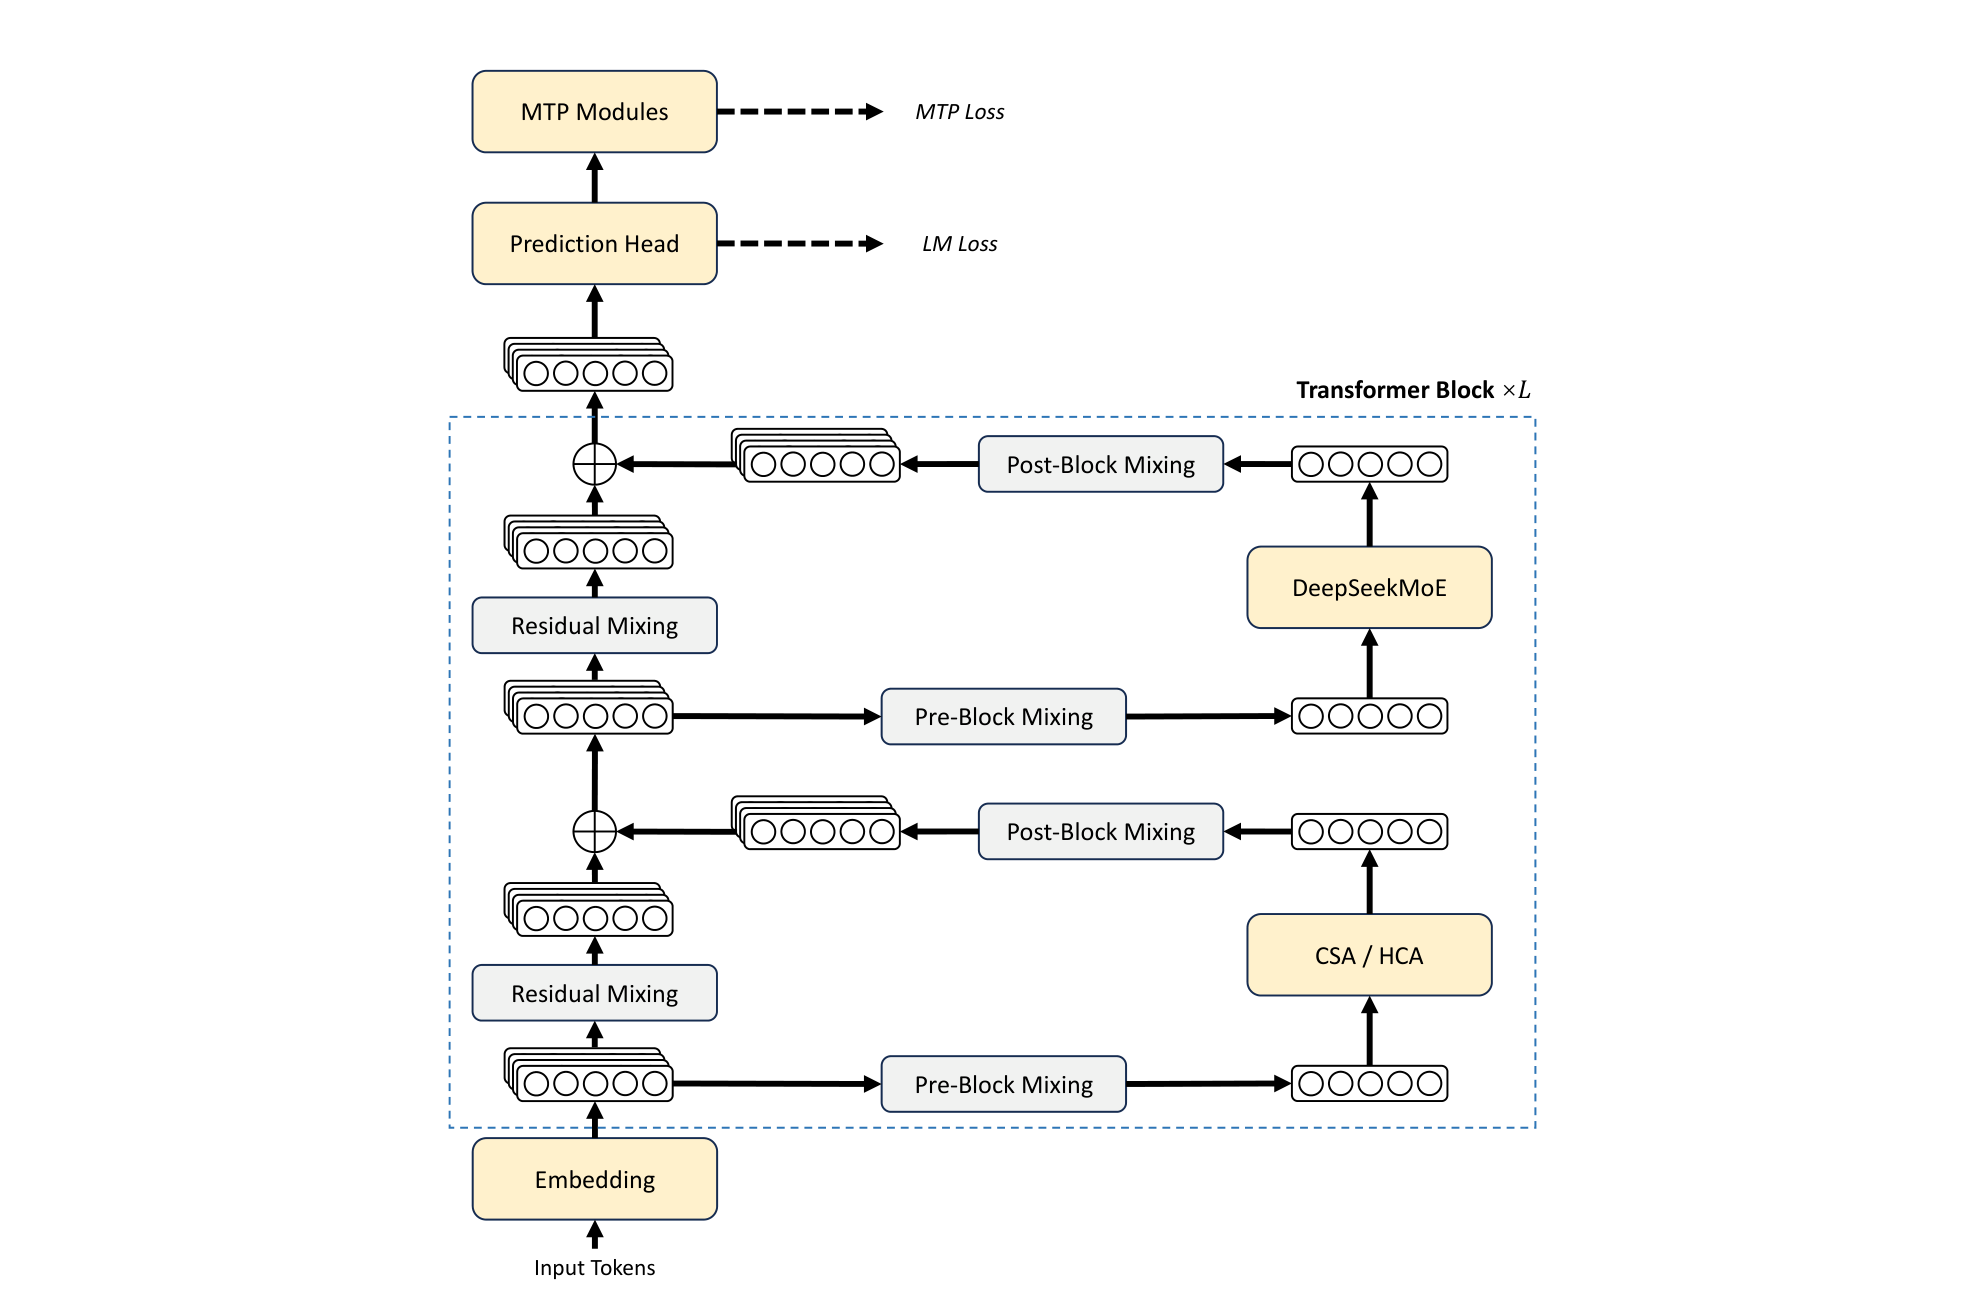
\includegraphics[width=\textwidth]{figures/DeepSeek_V4_fig02.png}
\caption{\dsvfour 系列整体架构。我们采用混合CSA（压缩稀疏注意力）和HCA（重度压缩注意力），并结合流形约束超连接（mHC）以及Muon优化器。}
\label{fig:arch}
\end{figure}

如图2所示，\dsvfour 系列融合了流形约束超连接（mHC），以增强相邻Transformer块之间的传统残差连接。与朴素的超连接（HC）相比，mHC的核心思想是将残差映射约束到一个特定的流形上，从而增强跨层信号传播的稳定性，同时保持模型的表现力。

\subsubsection*{标准超连接}
标准HC将残差流的宽度扩展\(n_{\mathrm{hc}}\)倍。具体来说，残差流的形状从\(\mathbb{R}^d\)扩展至\(\mathbb{R}^{n_{\mathrm{hc}}\times d}\)。令\(X_{l} = [\mathbf{x}_{l,1};\ldots ;\mathbf{x}_{l,n_{\mathrm{hc}}}]^{T}\in \mathbb{R}^{n_{\mathrm{hc}}\times d}\)为第\(l\)层之前的残差状态。HC引入三个线性映射：输入映射\(A_{l}\in \mathbb{R}^{1\times n_{\mathrm{hc}}}\)、残差变换\(B_{l}\in \mathbb{R}^{n_{\mathrm{hc}}\times n_{\mathrm{hc}}}\)和输出映射\(C_{l}\in \mathbb{R}^{n_{\mathrm{hc}}\times 1}\)。残差状态的更新公式如下：
\[X_{l+1} = B_{l}X_{l} + C_{l}\mathcal{F}_{l}(A_{l}X_{l}),\]
其中\(\mathcal{F}_{l}\)表示第\(l\)层，其输入和输出形状均为\(\mathbb{R}^d\)。HC将残差宽度与实际隐藏层大小解耦，提供了一个补充的扩展轴，且计算开销极小。然而，尽管HC已展现出提升模型性能的潜力，但我们发现当堆叠多层时，训练会频繁出现数值不稳定，这阻碍了HC的扩展。

\subsubsection*{流形约束残差映射}
mHC的核心创新在于将残差映射矩阵\(B_{l}\)约束到双随机矩阵流形（Birkhoff多面体）\(\mathcal{M}\)上，从而增强跨层信号传播的稳定性：
\[B_{l}\in \mathcal{M}\coloneqq \{M\in \mathbb{R}^{n\times n}\mid M\mathbf{1}_{n} = \mathbf{1}_{n},\mathbf{1}_{n}^{T}M = \mathbf{1}_{n}^{T},M\geqslant 0\} .\]
此约束确保映射矩阵的谱范数\(\| B_{l}\|_{2}\)以1为界，因此残差变换是非扩张的，这增加了前向传播和反向传播过程中的数值稳定性。此外，集合\(\mathcal{M}\)在乘法下是封闭的，这保证了深层mHC堆叠场景下的稳定性。另外，输入变换\(A_{l}\)和输出变换\(C_{l}\)也通过Sigmoid函数被约束为非负且有界，以避免信号抵消的风险。

\subsubsection*{动态参数化}
三个线性映射的参数是动态生成的，它们被分解为动态（输入相关）分量和静态（输入无关）分量。给定输入\(X_{l}\in \mathbb{R}^{n_{\mathrm{hc}}\times d}\)，它首先被展平并归一化：\(\hat{X}_{l} = \mathrm{RMSNorm}(\mathrm{vec}(X_{l}))\in \mathbb{R}^{1\times n_{\mathrm{hc}}d}\)。然后，我们按照传统HC生成无约束的原始参数\(\tilde{A}_{l},\tilde{B}_{l},\tilde{C}_{l}\)：
\[\begin{array}{rl} 
\tilde{A}_{l} &= \alpha_{l}^{\mathrm{pre}}\cdot (\hat{X}_{l}W_{l}^{\mathrm{pre}}) + S_{l}^{\mathrm{pre}},\\
\tilde{B}_{l} &= \alpha_{l}^{\mathrm{res}}\cdot \mathrm{Mat}(\hat{X}_{l}W_{l}^{\mathrm{res}}) + S_{l}^{\mathrm{res}},\\
\tilde{C}_{l} &= \alpha_{l}^{\mathrm{post}}\cdot (\hat{X}_{l}W_{l}^{\mathrm{post}})^{T} + S_{l}^{\mathrm{post}},
\end{array}\]
其中\(W\)为可学习参数，\(S\)为可学习静态偏置，\(\alpha\)为可学习门控因子。

\subsubsection*{应用参数约束}
获得原始参数后，我们对其施加约束以增强数值稳定性。对于输入和输出映射，我们采用Sigmoid函数\(\sigma(\cdot)\)确保非负性和有界性：
\[A_{l} = \sigma(\tilde{A}_{l}),\quad C_{l} = 2\sigma(\tilde{C}_{l}).\]
对于残差映射\(\tilde{B}_{l}\)，我们通过Sinkhorn-Knopp算法将其投影到双随机矩阵流形\(\mathcal{M}\)上。该算法首先对\(\tilde{B}_{l}\)应用指数函数以确保正性，得到\(M^{(0)} = \exp(\tilde{B}_{l})\)，然后迭代地执行行列归一化：
\[M^{(t)} = \mathcal{T}_{r}(\mathcal{T}_{c}(M^{(t-1)})),\]
其中\(\mathcal{T}_{r}\)和\(\mathcal{T}_{c}\)分别表示行和列归一化。此迭代收敛于受约束的双随机矩阵\(B_{l} = M^{(t_{\mathrm{max}})}\)。我们选择\(t_{\mathrm{max}} = 20\)作为实用值。

\subsection{CSA与HCA混合注意力}

随着上下文长度达到极限规模，注意力机制成为模型中的主导计算瓶颈。对于\dsvfour，我们设计了两种高效的注意力架构——压缩稀疏注意力和重度压缩注意力——并采用它们的交错混合配置，这大幅降低了长文本场景下注意力的计算成本。

\subsubsection{压缩稀疏注意力}

\begin{figure}[H]
\centering
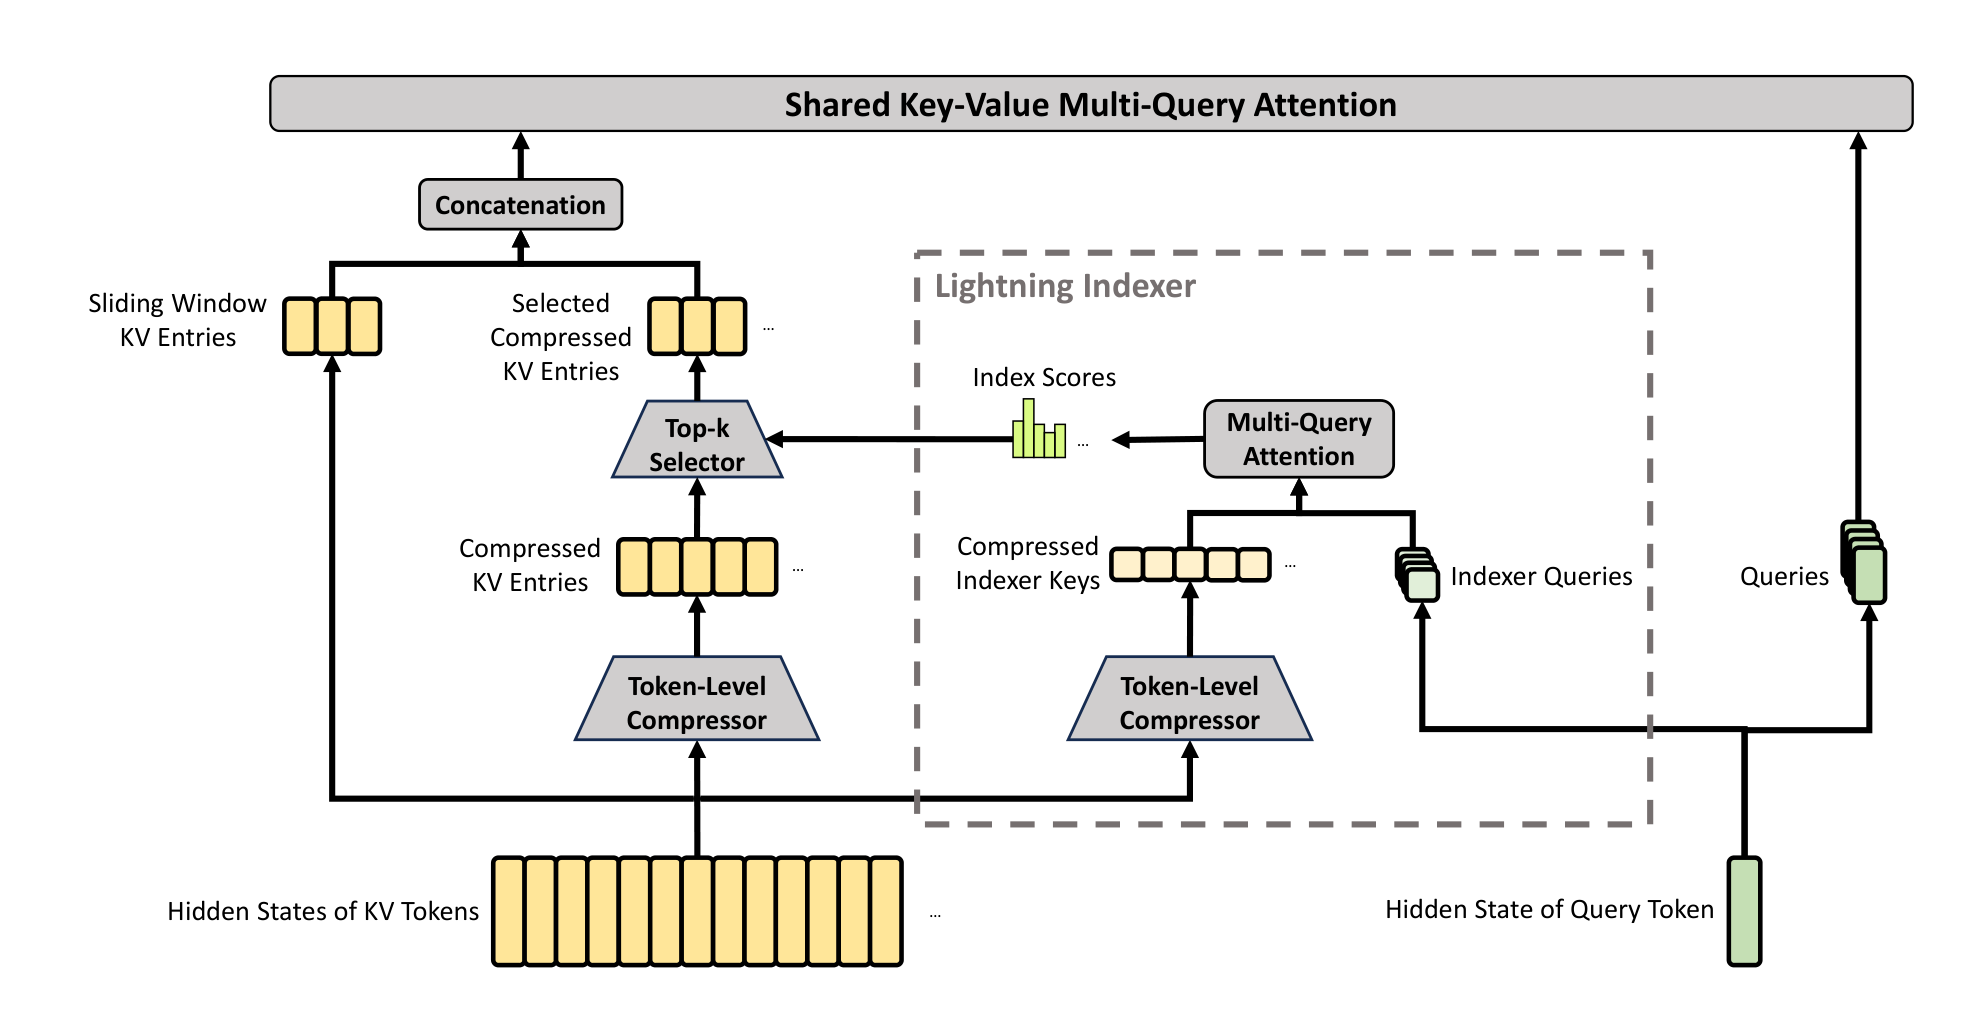
\includegraphics[width=\textwidth]{figures/DeepSeek_V4_fig03.png}
\caption{CSA（压缩稀疏注意力）核心架构。它将KV条目数压缩至\(1/m\)倍，并应用DeepSeek稀疏注意力进一步加速。}
\label{fig:csa}
\end{figure}

CSA的核心架构如图3所示，它首先将每\(m\)个Token的KV缓存压缩成一个条目，然后应用DeepSeek稀疏注意力以进一步加速。

\textbf{压缩键值条目。} 令\(H\in \mathbb{R}^{n\times d}\)为输入隐藏状态序列。CSA首先计算两个KV条目序列\(C^a,C^b\in \mathbb{R}^{n\times c}\)及其对应的压缩权重\(Z^{a},Z^{b}\in \mathbb{R}^{n\times c}\)，其中\(c\)为头维度。接下来，\(C^a\)和\(C^b\)中每\(m\)个KV条目将根据其压缩权重和可学习位置偏置\(B^a,B^b\in \mathbb{R}^{m\times c}\)被压缩成一个条目，生成\(C^{\mathrm{Comp}}\in \mathbb{R}^{\frac{n}{m}\times c}\)。注意，每个\(C_i^{\mathrm{Comp}}\)由\(2m\)个KV条目导出，但用于\(C_i^{\mathrm{Comp}}\)的\(C^b\)索引与用于\(C_{i-1}^{\mathrm{Comp}}\)的\(C^a\)索引存在重叠。因此，CSA实际上将序列长度压缩至\(\frac{1}{m}\)倍。

\textbf{用于稀疏选择的闪电索引器。} 在获得压缩KV条目\(C^{\mathrm{Comp}}\)后，CSA应用DSA策略选择top-k压缩KV条目用于核心注意力。首先，CSA执行与\(C^{\mathrm{Comp}}\)相同的压缩操作以获得压缩索引器键\(K^{\mathrm{Comp}}\in \mathbb{R}^{\frac{n}{m}\times c^l}\)。然后，对于查询Token \(t\)，我们以低秩方式生成索引器查询\(\{\mathbf{q}_{t,1}^{l};\dots;\mathbf{q}_{t,n_h^l}^{l}\}\)：
\[\mathbf{c}_t^Q = \mathbf{h}_t\cdot W^{DQ},\quad [\mathbf{q}_{t,1}^I;\dots;\mathbf{q}_{t,n_h^I}^I] = \mathbf{q}_t^I = \mathbf{c}_t^Q\cdot W^{IUQ}.\]
接下来，查询Token \(t\)与之前的压缩块\(s\)之间的索引分数\(I_{t,s}\)计算为：
\[[w_{t,1}^{I};\dots ;w_{t,n_h^{I}}^{I}] = \mathbf{w}_{t}^{I} = \mathbf{h}_{t}\cdot W^{w},\quad I_{t,s} = \sum_{h=1}^{n_h^{I}}w_{t,h}^{I}\cdot \mathrm{ReLU}\left(\mathbf{q}_{t,h}^{I}\cdot K_{s}^{\mathrm{Comp}}\right).\]
然后，采用top-k选择器保留一个压缩KV条目的子集\(C_t^{\mathrm{SprsComp}}\)用于后续核心注意力。

\textbf{分組输出投影。} 在\dsvfour 的配置中，\(cn_h\)非常大。为降低计算负担，我们设计了一种分组输出投影策略。我们将\(n_h\)个输出分成\(g\)组，每组输出\(\mathbf{o}_{t,i}^G\in \mathbb{R}^{c\frac{n_h}{g}}\)被投影到\(d_g\)维中间输出\(\mathbf{o}_{t,i}^{G'}\in \mathbb{R}^{d_g}\)。最后，我们将中间输出投影到维度为\(d\)的最终注意力输出。

\subsubsection{重度压缩注意力}

\begin{figure}[H]
\centering
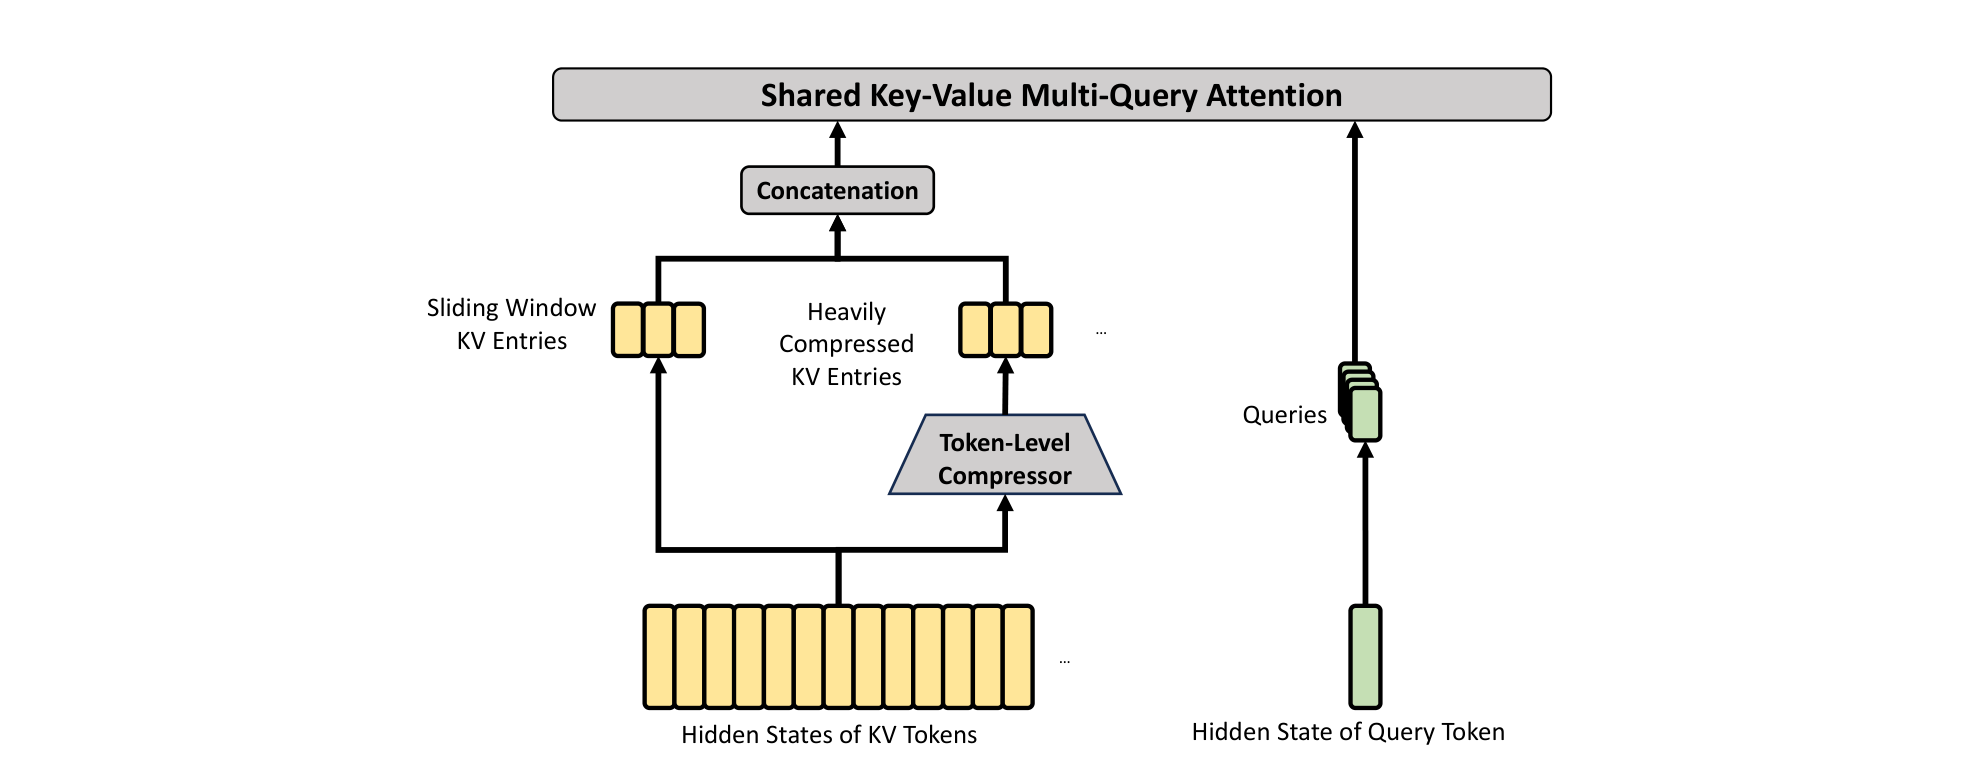
\includegraphics[width=\textwidth]{figures/DeepSeek_V4_fig04.png}
\caption{HCA（重度压缩注意力）核心架构。它以更大的压缩率\(m'(\gg m)\)压缩KV缓存，并执行密集注意力。}
\label{fig:hca}
\end{figure}

HCA的核心架构如图4所示，它以更大的压缩率\(m'(\gg m)\)压缩KV缓存，但不采用稀疏注意力，而是进行密集注意力。

\subsubsection{其他细节}

\textbf{部分旋转位置嵌入。} 对于CSA和HCA，我们部分地对注意力查询、KV条目和核心注意力输出使用旋转位置嵌入（RoPE）。具体来说，我们对每个查询向量和KV条目的最后64维应用RoPE。由于KV条目同时充当注意力键和值，初始核心注意力输出会携带绝对位置嵌入。作为对策，我们还对每个\(\mathbf{o}_{t,i}\)的最后64维应用位置\(-i\)的RoPE。

\textbf{滑动窗口注意力的附加分支。} 为了严格保持CSA和HCA中的因果性，每个查询只能关注之前的压缩KV块。因此，查询无法访问其自身压缩块内其他Token的信息。同时，近期Token在语言建模中通常与查询Token具有更大的相关性。出于这些原因，我们为CSA和HCA都引入了一个滑动窗口方式的补充注意力分支。具体来说，对于每个查询Token，我们额外生成对应于最近\(n_{\mathrm{win}}\)个Token的未压缩KV条目。在CSA和HCA的核心注意力中，这些滑动窗口中的KV条目将与压缩KV条目一起使用。

\textbf{注意力汇}。在CSA和HCA的核心注意力中，我们采用了注意力汇技巧。具体来说，我们设置了一系列可学习的汇Logits \(\{z_{1}^{\prime},\dots,z_{n_h}^{\prime}\}\)。对于第\(h\)个注意力头，\(\mathrm{Exp}(z_{h}^{\prime})\)将被加到注意力分数的分母中：
\[s_{h,i,j} = \frac{\mathrm{Exp}(z_{h,i,j})}{\sum_{k}\mathrm{Exp}(z_{h,i,k}) + \mathrm{Exp}(z_{h}^{\prime})}.\]
此技术允许每个查询头调整其总注意力分数使其不等于1，甚至可接近0。

\subsubsection{效率讨论}

由于采用混合CSA和HCA，以及低精度计算和存储，\dsvfour 系列的注意力模块在注意力FLOPs和KV缓存大小方面都实现了显著效率，尤其在长上下文场景下。首先，我们对KV条目采用混合存储格式：旋转位置嵌入维度使用BF16精度，其余维度使用FP8精度。与纯BF16存储相比，这种混合表示将KV缓存大小减少了近一半。其次，闪电索引器中的注意力计算以FP4精度执行，这加速了超长上下文下的注意力操作。第三，相对于\dsvthreetwo，\dsvfour 系列选择了更小的注意力top-k，从而提高了短文本和中文本上的模型效率。最后，也是最重要的，压缩注意力和混合注意力技术大幅减少了KV缓存大小和计算FLOPs。

以BF16 GQA8，头维度128作为基线——这是LLM注意力的常见配置之一——在1M上下文设置下，\dsvfour 系列的KV缓存大小可被大幅降低至该基线的约\(2\%\)。此外，即使与已经是高效基线的\dsvthreetwo 相比，\dsvfour 系列仍然展现出显著的效率优势。

\subsection{Muon优化器}

由于收敛速度更快且训练稳定性得到改善，我们对\dsvfour 系列中的大多数模块采用Muon优化器。

\begin{algorithm}
\caption{Muon优化}
\begin{algorithmic}[1]
\For{每个训练步 \(t\)}
    \For{每个逻辑上独立的权重 \(W \in \mathbb{R}^{n \times m}\)}
        \State \(G_{t} = \nabla_{W} \mathcal{L}_{t}(W_{t-1})\) \Comment{计算梯度}
        \State \(M_{t} = \mu M_{t-1} + G_{t}\) \Comment{累积动量缓冲区}
        \State \(O_{t}^{\prime} = \text{HybridNewtonSchulz}(\mu M_{t} + G_{t})\) \Comment{Nesterov技巧与混合Newton-Schulz}
        \State \(O_{t} = O_{t}^{\prime} \cdot \sqrt{\max(n, m)} \cdot \gamma\) \Comment{重新缩放更新RMS}
        \State \(W_{t} = W_{t-1} \cdot (1 - \eta \lambda) - \eta O_{t}\) \Comment{执行权重衰减和更新}
    \EndFor
\EndFor
\end{algorithmic}
\end{algorithm}

\textbf{混合Newton-Schulz迭代。} 对于一个给定的矩阵\(M\)，其SVD为\(M = U \Sigma V^{T}\)。Newton-Schulz迭代旨在将\(M\)近似正交化为\(UV^{T}\)。通常，\(M\)将首先被归一化为\(M_{0} = M / ||M||_{F}\)。每次迭代执行：
\[M_{k} = a M_{k-1} + b(M_{k-1} M_{k-1}^{T}) M_{k-1} + c(M_{k-1} M_{k-1}^{T})^{2} M_{k-1}.\]
我们的混合Newton-Schulz在两个不同阶段执行10次迭代。在前8步中，我们使用系数\((a, b, c) = (3.4445, -4.7750, 2.0315)\)以驱动快速收敛。在最后2步中，我们切换至\((a, b, c) = (2, -1.5, 0.5)\)，以将奇异值精确稳定在1。

\textbf{避免注意力Logits爆炸。} \dsvfour 系列的注意力架构允许我们直接对注意力查询和KV条目应用RMSNorm，这有效防止了注意力Logits爆炸。因此，我们在Muon优化器中不使用QK-Clip技术。

% ===== 3. 通用基础设施 =====
\section{通用基础设施}

\subsection{专家并行中细粒度的通信-计算重叠}
混合专家（\moe{}）可通过专家并行（EP）加速。然而，EP需要复杂的节点间通信，并对互连带宽和延迟提出很高要求。为缓解EP中的通信瓶颈并在较低互连带宽要求下实现更高的端到端性能，我们提出了一种细粒度的EP方案，将通信和计算融合到单个流水线化内核中，实现通信-计算重叠。

\textbf{可隐藏的通信延迟。} 我们的EP方案的关键洞察在于，在\moe{}层中，通信延迟可以有效地隐藏在计算之下。在\dsvfour 系列中，每个\moe{}层主要可分解为四个阶段：两个通信密集型阶段（分发和合并）以及两个计算密集型阶段（线性1和线性2）。我们的分析显示，在单个\moe{}层中，总通信时间少于计算时间。因此，将通信和计算融合到统一流水线后，计算仍然是主要瓶颈，这意味着系统可以在不降低端到端性能的情况下容忍较低的互连带宽。

\textbf{细粒度EP方案。} 为进一步降低互连带宽需求并放大重叠的好处，我们引入了一种更细粒度的专家划分方案。我们拆分专家并按波次调度。每个波次包含一小部分专家。当一个波次内的所有专家完成其通信后，计算可以立即开始，无需等待其他专家。在稳态下，当前波次的计算、下一波次的Token传输以及已完成专家的结果发送均并发进行。

\textbf{性能与开源的Mega-Kernel。} 我们在NVIDIA GPU和华为昇腾NPU平台上验证了细粒度EP方案。与强非融合基线相比，它在通用推理工作负载上实现了\(1.50 \sim 1.73 \times\)的加速，对于RL推理和高速Agent服务等延迟敏感场景，加速比可达\(1.96 \times\)。我们已将基于CUDA的Mega-Kernel实现开源，命名为MegaMoE，作为DeepGEMM的一部分。

\subsection{使用TileLang进行灵活高效的Kernel开发}
我们采用TileLang来开发一组融合Kernel，以替换绝大多数细粒度的Torch ATen算子，用最少的工作量提供最佳性能。作为领域特定语言，TileLang平衡了开发效率与运行时效率，支持在同一代码库内进行快速开发和深度迭代优化。

\subsection{高性能批次不变与确定性Kernel库}
为保障训练的可复现性以及预训练、后训练和推理管线之间的逐位对齐，我们实现了端到端的、逐位批次不变的确定性Kernel，且性能开销极小。

\textbf{批次不变性。} 批次不变性确保任何给定Token的输出保持逐位一致，无论其在批次中的位置如何。注意力机制方面，我们开发了用于批次不变解码的双Kernel策略。第一个Kernel在单个SM上计算整个序列的注意力输出。第二个Kernel旨在最小化最后部分填充波次的延迟，使用多个SM处理单个序列，并仔细设计计算路径以确保与第一个Kernel的累加顺序相同。

\textbf{确定性。} 确定性训练对于调试硬件或软件问题非常有益。训练中的非确定性通常源于非确定性的累加顺序。我们在注意力反向传播、\moe{}反向传播以及mHC中的矩阵乘法等部分设计了特定策略，以在保持性能的同时确保确定性。

\subsection{FP4量化感知训练}
为在部署时实现推理加速和内存节省，我们在后训练阶段引入量化感知训练（QAT），使模型能够适应量化引入的精度损失。我们将FP4量化应用于\moe{}专家权重和CSA索引器中的查询-键路径。此外，在此QAT过程中，我们还将索引分数从FP32量化到BF16，为top-k选择器实现了\(2\times\)加速，同时保持了\(99.7\%\)的KV条目召回率。

\subsection{训练框架}
我们的训练框架建立在为\dsvthree 开发的可扩展高效基础设施之上。为适应\dsvfour 中的Muon优化器、mHC和混合注意力机制，我们引入了若干关键创新。

\subsubsection{高效实现Muon}
Muon优化器需要完整的梯度矩阵来计算参数更新，这与ZeRO存在冲突。我们为Muon设计了ZeRO桶分配的混合策略。对于密集参数，我们限制ZeRO并行的最大规模，并采用背包算法分配参数矩阵以确保负载均衡。对于\moe{}参数，我们独立优化每个专家，展平所有专家、所有层的投影矩阵，然后在不拆分任何逻辑独立矩阵的情况下将其平均分配。

\subsubsection{高性价比且内存高效的mHC实现}
mHC的引入增加了激活内存消耗和流水线阶段间的通信量。为降低成本，我们实现了mHC的融合Kernel，引入了选择性检查点中间张量的重计算策略，并调整了DualPipe 1F1B重叠方案以适应增加的流水线通信。

\subsubsection{用于长上下文注意力的上下文并行}
传统上下文并行（CP）对序列维度进行划分。这对我们的压缩注意力机制提出了两个挑战：各rank的压缩KV长度不一致，且压缩可能跨越相邻CP rank的边界。为应对这些挑战，我们设计了一种两阶段通信方法。第一阶段在各rank间发送未压缩KV条目，第二阶段通过all-gather收集并在本地压缩，最终重组成完整的压缩KV条目集合。

\subsubsection{扩展自动微分以实现灵活激活检查点}
为实现精细控制而不牺牲编程效率，我们在自动微分支持下实现了张量级激活检查点机制。开发者只需实现前向传播，并有选择地注释个别张量以进行自动检查点和重计算。我们的框架利用TorchFX追踪完整计算图，并识别重计算所需的最小子图。

\subsection{推理框架}
我们的推理框架主要继承自\dsvthree，但在KV缓存管理方面存在一些差异。

\subsubsection{KV缓存结构与管理}
为高效管理由混合注意力机制产生的异构KV缓存，我们设计了一种定制的KV缓存布局。

\textbf{用于SWA和未压缩尾部Token的状态缓存。} 由于SWA和压缩分支的未压缩尾部Token可被视为状态空间模型，其对应的KV缓存可看作仅依赖于当前位置的序列特定状态。因此，我们预分配固定且大小有限的状态缓存池，并动态分配给每个序列。

\textbf{稀疏注意力内核协同设计。} 传统高性能注意力内核通常假设每块固定\(B\)个Token以优化性能。通过使用高性能稀疏注意力内核，不同层可以在不降低性能的情况下容纳每块可变数量的Token。

\subsubsection{磁盘KV缓存存储}
在服务\dsvfour 时，我们利用磁盘KV缓存存储机制来消除共享前缀请求的重复预填充。对于CSA/HCA中的压缩KV条目，我们直接将其存储到磁盘。对于SWA的KV条目，我们提出并实现了三种不同的管理策略：全量SWA缓存、周期性检查点和零SWA缓存，每种策略在存储开销和计算冗余之间提供了不同的权衡。

% ===== 4. 预训练 =====
\section{预训练}

\subsection{数据构建}
在\dsvthree 预训练数据的基础上，我们致力于构建一个更多样化、更高质量、且具有更长有效上下文的训练语料库。我们不断改进数据构建流程。对于网络数据，我们实施过滤策略以移除批量自动生成和模板化的内容。数学和编程语料仍然是核心，我们通过在中训练阶段加入智能体数据来进一步增强编码能力。对于多语言数据，我们构建了更大的语料库以改善其对不同文化长尾知识的捕获。我们对长文档数据策展给予特别强调，优先考虑科学论文、技术报告等反映独特学术价值的材料。综上，我们的预训练语料库包含超过32T Token。

\subsection{预训练设置}

\subsubsection{模型设置}

\textbf{\dsvfourflash}。Transformer层数61，隐藏维度7168。前两层使用HCA，其余层交错使用CSA和HCA。CSA压缩率\(m=4\)，索引器查询头数64，头维度128，稀疏注意力选择的KV条目数1024。HCA压缩率\(m'=128\)。查询头数128，头维度512，查询压缩维度1536。输出投影组数16，中间注意力输出维度1024。滑动窗口大小128。所有Transformer块使用\moe{}层，前3个\moe{}层使用哈希路由。每个\moe{}层包含1个共享专家和384个路由专家，每个Token激活6个专家。多Token预测深度1。mHC扩展因子4，Sinkhorn迭代20。在此配置下，总参数1.6T，每Token激活49B。

\textbf{\dsvfourpro}。Transformer层数43，隐藏维度4096。前两层使用纯滑动窗口注意力，其余层交错使用CSA和HCA。CSA压缩率\(m=4\)，索引器查询头数64，头维度128，注意力top-k为512。HCA压缩率\(m'=128\)。查询头数64，头维度512，查询压缩维度1024。输出投影组数8，中间注意力输出维度1024。滑动窗口大小128。所有Transformer块使用\moe{}层，前3个\moe{}层使用哈希路由。每个\moe{}层包含1个共享专家和256个路由专家，每个Token激活6个专家。多Token预测深度1。总参数284B，每Token激活13B。

\subsubsection{训练设置}

\textbf{\dsvfourflash}。大多数参数使用Muon优化器，嵌入模块、预测头模块和所有RMSNorm模块的权重使用AdamW。训练32T Token，采用批次大小调度策略，最大批次大小75.5M。学习率在首2000步线性预热，大部分训练维持在\(2.7 \times 10^{-4}\)，最后按余弦计划衰减至\(2.7 \times 10^{-5}\)。序列长度从4K逐步扩展到16K、64K和1M。在首1T Token使用密集注意力热身，在64K序列长度时引入稀疏注意力。

\textbf{\dsvfourpro}。训练设置与Flash大体一致。训练33T Token，最大批次大小94.4M。峰值学习率\(2.0 \times 10^{-4}\)，最终学习率\(2.0 \times 10^{-5}\)。序列长度同样逐步扩展至1M，密集注意力热身的阶段更长。

\subsubsection{缓解训练不稳定性}

训练万亿参数\moe{}模型面临显著的稳定性挑战。我们遇到了显著的训练不稳定问题。我们发现了两种实用的技术来有效维持训练稳定性：前瞻性路由和SwiGLU Clamping。

\textbf{前瞻性路由}。我们发现解耦骨干网络和路由网络的同步更新显著提升了训练稳定性。因此，在步\(t\)，我们使用当前网络参数\(\theta_t\)进行特征计算，但路由索引使用历史参数\(\theta_{t-\Delta t}\)计算和应用。我们实现了基础设施层面的深度优化，将额外的墙钟时间开销控制在约\(20\%\)。

\textbf{SwiGLU Clamping}。我们凭经验发现，应用SwiGLU Clamping能有效消除异常值，并极大地帮助稳定训练过程。在整个训练过程中，我们将SwiGLU的线性分量约束在\([-10,10]\)范围内，同时将门控分量的上限限制在10。

\subsection{评估}

\subsubsection{评估基准}
评估涵盖世界知识、语言理解与推理、编码与数学以及长上下文处理四个关键维度。

\subsubsection{评估结果}
在统一内部框架下的对比显示，\dsvfourflash-Base尽管使用的激活和总参数数量少得多，但在广泛基准上超越了\dsvthreetwo-Base，在知识任务和长上下文场景上优势尤为明显。\dsvfourpro-Base在此基础上进一步实现了决定性的能力飞跃，几乎在所有类别上对\dsvthreetwo-Base和\dsvfourflash-Base都建立了普遍优势，成为DeepSeek系列中最强大的基础模型。

% ===== 5. 后训练 =====
\section{后训练}

\subsection{后训练流程}
遵循预训练，我们进行后训练以得到最终模型。训练流程大体模拟了\dsvthreetwo，但一个关键的方法论替代是：混合强化学习阶段完全被在线策略蒸馏所取代。

\subsubsection{专家训练}
领域专家的发展通过改造\dsvthreetwo 训练流程进行。每个模型依次通过初始微调和后续的（RL）进行优化。RL阶段实施GRPO算法。

\textbf{推理努力}。我们为\dsvfourpro 和\dsvfourflash 训练了不同的专家模型，以支持三种特定的推理努力模式：Non-think、Think High和Think Max。对于每种模式，我们在RL训练期间应用不同的长度惩罚和上下文窗口，导致推理的输出Token长度不同。对于“Think Max”模式，我们在系统提示开头注入特定指令来引导推理过程。

\textbf{生成式奖励模型}。通常，易于验证的任务可使用简单的规则验证器。对于难以验证的任务，我们不使用传统的标量奖励模型，而是策展指导性RL数据并采用生成式奖励模型（GRM）来评估策略轨迹。关键的是，我们直接对GRM本身应用RL优化。在此范式中，Actor网络原生地充当GRM，实现了模型评估能力与其标准生成能力的联合优化。

\textbf{工具调用模式与特殊Token}。我们利用专门的<think></think>标签来描绘推理路径。我们引入了一种新的工具调用模式，使用特殊的“|DSML|”Token，并利用基于XML的格式进行工具调用。

\textbf{交错思考}。\dsvthreetwo 引入了一种上下文管理策略，在工具结果轮次保留推理轨迹，而在新用户消息到达时将其丢弃。利用\dsvfour 系列扩展的1M Token上下文窗口，我们进一步细化了此机制以最大化智能体环境中交错思考的有效性。在工具调用场景中，所有推理内容在整个对话中都被完全保留。在通用对话场景中，保留原始策略。

\textbf{快速指令}。在聊天机器人场景中，必须在生成响应之前执行许多辅助任务（例如，确定是否触发网络搜索）。为克服这一限制，我们引入了快速指令。我们将一组专用的特殊Token直接附加到输入序列，通过直接重用已计算的KV缓存，完全避免了冗余预过滤。

\subsubsection{在线策略蒸馏}
在通过专门微调和RL训练多个领域专家后，我们采用多教师在线策略蒸馏（OPD）作为将专家能力合并到最终模型的主要技术。给定一组\(N\)个专家模型\(\{\pi_{E_1},\dots,\pi_{E_N}\}\)，OPD目标函数定义为：
\[\mathcal{L}_{\mathrm{OPD}}(\theta) = \sum_{i=1}^{N}w_{i}\cdot \mathrm{D}_{\mathrm{KL}}\left(\pi_{\theta}\parallel \pi_{E_{i}}\right).\]
我们没有将完整词汇KL损失简化为Token级KL估计，而是采用完整词汇Logits蒸馏，以产生更稳定的梯度估计并确保对教师知识的忠实蒸馏。

\subsection{RL与OPD基础设施}
\subsubsection{FP4量化集成}
我们应用FP4量化来加速rollout以及所有仅推理前向传播，包括教师和参考模型的前向传播。我们直接在rollout和推理阶段使用原生FP4权重。对于训练步，通过无损的FP4到FP8反量化步骤模拟FP4量化，无缝重用了现有的FP8混合精度框架。

\subsubsection{用于完整词汇OPD的高效教师调度}
我们的框架支持具有几乎无限数量教师的完整词汇OPD。所有教师权重被卸载到集中式分布式存储，并在需要时加载。我们通过在教师前向传播期间仅缓存最后一层教师隐藏状态，并在训练时重建成完整的Logits来解决显式Logits实体化带来的内存负担。为减轻教师预测头的GPU内存占用，我们在数据分发期间按教师索引对训练样本进行排序。

\subsubsection{可抢占与容错的Rollout服务}
为最大化GPU资源利用率，我们的集群采用全集群抢占式任务调度器。同时，硬件故障普遍存在。为此，我们为RL/OPD rollout实现了一个可抢占和容错的大语言模型生成服务。具体而言，我们为每个生成请求实现了Token粒度预写日志（WAL）。任何已生成的Token都会被立即追加到WAL。在抢占发生时，我们暂停推理引擎并保存未完成请求的KV缓存。恢复时，使用持久化的WAL和保存的KV缓存继续解码。重要的是，从头重新生成未完成的请求在数学上是不正确的，因为这会引入长度偏差。

\subsubsection{为百万级Token扩展RL框架}
针对百万级Token序列上的高效RL和OPD，我们引入了针对性优化。在rollout阶段，我们采用可抢占和容错的rollout服务。在推理和训练阶段，我们将rollout数据格式分解为轻量级元数据和重量级逐Token字段。重量级字段通过共享内存数据加载器加载以消除节点内数据冗余，并在消费后立即释放。

\subsubsection{面向智能体AI的沙箱基础设施}
为满足后训练和评估中智能体AI的多样化执行需求，我们构建了一个生产级沙箱平台DeepSeek Elastic Compute (DSec)。DSec的设计基于四个观察：（1）智能体工作负载高度异构；（2）环境镜像数量多、体积大，但必须快速加载并支持迭代定制；（3）高密度部署要求高效利用CPU和内存；（4）沙箱生命周期必须与GPU训练计划协调。

\textbf{统一接口下的四种执行基板。} DSec暴露一个单一的Python SDK(libdsec)，抽象了四种执行基板：函数调用、容器、microVM和fullVM，只需更改参数即可在它们之间切换。

\textbf{通过分层存储实现快速镜像加载。} DSec通过分层的按需加载协调了快速启动与不断增长的环境镜像库。对于容器，基础镜像和文件系统提交存储为3FS支持的只读EROFS层。

\textbf{大规模并发下的密度优化。} 为容纳每集群数十万个沙箱，DSec解决了两个资源瓶颈：减轻虚拟化环境中的重复页缓存占用并应用内存回收，以及减轻容器运行时中的自旋锁争用。

\textbf{轨迹记录与抢占安全恢复。} DSec为每个沙箱维护一个全局有序的轨迹日志，持久化记录每条命令调用及其结果。

\subsection{标准基准评估}
\subsubsection{评估设置}
评估涵盖知识和推理、1M Token上下文和智能体等数据集。对于代码，我们评估LiveCodeBench-v6和我们内部的Codeforces基准。对于推理和知识任务，我们设置温度1.0，上下文窗口根据模式设为8K、128K或384K。对于形式化数学任务，我们在Lean 4.28.0-rcl上以智能体设置进行评估。

\subsubsection{评估结果}
在知识评估中，\dsvfourpromax 在开源大语言模型中建立了新的技术前沿。在推理方面，\dsvfourpromax 在所有推理基准上超越了以往的所有开源模型。在代码竞赛中，\dsvfourpro 和\dsvfourflash 表现出色，性能可与GPT-5.4相媲美。在智能体评估中，\dsvfour 系列展示了强大的性能。在1M Token上下文方面，\dsvfourpro 在MRCR任务上超越了Gemini-3.1-Pro，在CorpusQA上也表现出更好的性能。

\subsection{真实世界任务性能}
我们开发了专有的内部指标，优先考虑真实世界使用模式而非传统基准。

\subsubsection{中文写作}
中文写作是DeepSeek的主要用例之一。我们对功能写作和创意写作进行了严格评估。结果显示，\dsvfourpro 在功能写作上以\(62.7\%\)对\(34.1\%\)的总体胜率优于Gemini-3.1-Pro。在创意写作上，\dsvfourpro 在写作质量上取得了\(77.5\%\)的胜率，在指令遵循上为\(60.0\%\)。

\subsubsection{搜索}
在DeepSeek网站和应用上，“非思考”模式采用检索增强搜索（RAG），而“思考”模式利用智能体搜索。与\dsvthreetwo 相比，\dsvfourpro 在客观和主观问答类别上均大幅领先。智能体搜索在所有复杂性任务上始终优于标准RAG。

\subsubsection{白领任务}
为严格评估模型在复杂企业生产力场景下的实用性，我们构建了一套包含30个高级中文专业任务的套件，覆盖13个关键行业。人工评估结果显示，\dsvfourpromax 在多样化中文白领任务上优于Opus-4.6-Max，取得了\(63\%\)的不败率。

\subsubsection{代码智能体}
我们从内部研发工作负载中挑选任务来对编码智能体能力进行基准测试。评估集包含30个任务，跨度涵盖特性开发、Bug修复、重构和诊断。结果显示，\dsvfourpro 显著优于Claude Sonnet 4.5，并接近Claude Opus 4.5的水平。在一项对85名内部开发者和研究人员的调查中，超过\(52\%\)的人认为\dsvfourpro 已准备好作为其默认和主要的编码模型。

% ===== 6. 结论、局限与未来方向 =====
\section{结论、局限与未来方向}

在此工作中，我们呈现了\dsvfour 系列的预览版本，旨在实现突破超长上下文处理效率壁垒的下一代大语言模型。通过结合集成CSA和HCA的混合注意力架构，\dsvfour 系列在长序列效率上取得了巨大飞跃。架构创新与广泛的基础设施优化一道，使百万级Token上下文的高效原生支持成为可能，并为未来的测试时扩展、长程任务和如在线学习等新兴范式奠定了必要基础。评估结果表明，\dsvfourpromax 重新定义了开源模型的技术前沿。与此同时，\dsvfourflashmax 在保持高性价比架构的同时，取得了与领先闭源模型可比的推理性能。我们相信，\dsvfour 系列为开源模型开创了百万级上下文的新纪元，并铺平了通往更高效率、更大规模和更强智能的道路。

在追求极端长上下文效率的过程中，\dsvfour 系列采用了一种大胆的架构设计。为最小化风险，我们保留了许多初步验证过的组件和技巧，这使得架构相对复杂。在未来的迭代中，我们将进行更全面和原理性的研究，以提炼出最本质的设计，使其在不牺牲性能的前提下更加优雅。同时，尽管前瞻性路由和SwiGLU Clamping已被证明在缓解训练不稳定性方面有效，但其底层原理仍未被充分理解。我们将积极研究训练稳定性的基础问题，并加强内部指标监控，旨在以更系统化和可预测的方法实现稳定的大规模训练。

此外，除了\moe{}和稀疏注意力架构，我们还将积极探索沿新维度的模型稀疏性——例如更稀疏的嵌入模块——以在不损失能力的情况下进一步提高计算和内存效率。我们也将持续研究低延迟架构和系统技术，使长上下文部署和交互更加灵敏。此外，我们认识到长程、多轮智能体任务的重要性和实用价值，并将在此方向上持续迭代和探索。我们还在努力为我们的模型加入多模态能力。最后，我们致力于开发更好的数据策展和合成策略，以在日益广泛的场景和任务中持续增强模型的智能、鲁棒性和实用可用性。

\end{document}